\section{Cartes}

\subsection{Carte IHM}
\begin{frame}
    \frametitle{Carte IHM - \textcolor{green}{Terminée}}
    La carte IHM (Interface Homme-Machine) va nous permettre de sélectionner grâce aux boutons poussoirs de sélectionner le programme désiré. Les LEDs s'allumeront ensuite pour prévenir que le programme est lancé.

    \vfill
    \begin{figure}[H]
        \centering
        \begin{minipage}{.5\textwidth}
            \centering
            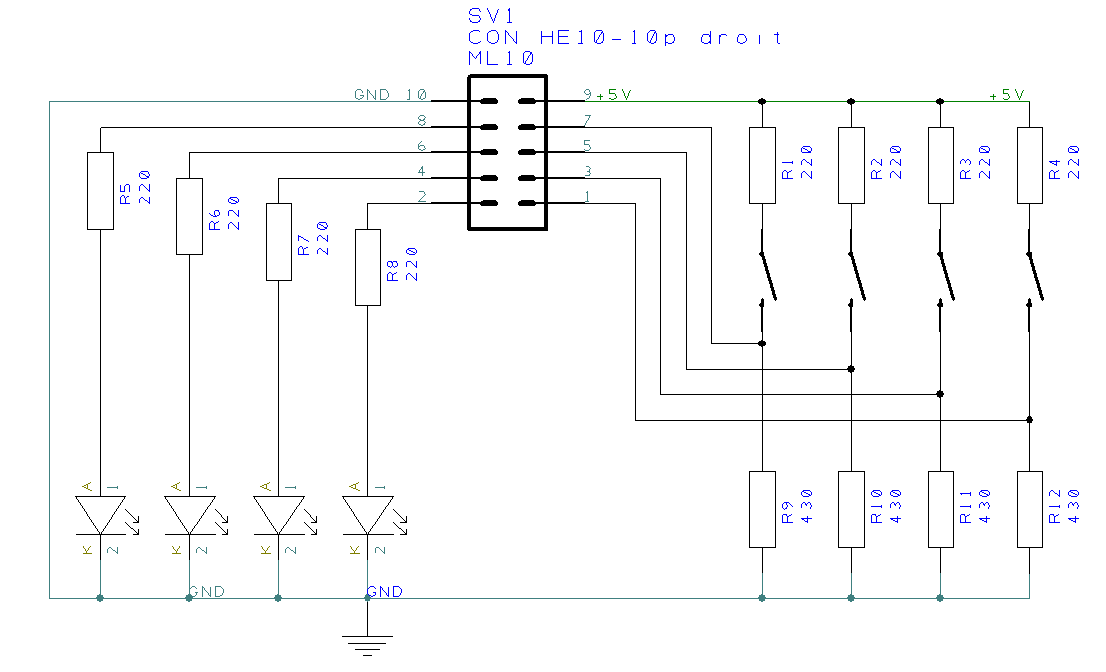
\includegraphics[width=.7\linewidth]{Images/carteIHM_sch.png}
            \caption{Carte IHM - Schématic}
            \label{fig:ihmsch}
        \end{minipage}%
        \begin{minipage}{.5\textwidth}
            \centering
            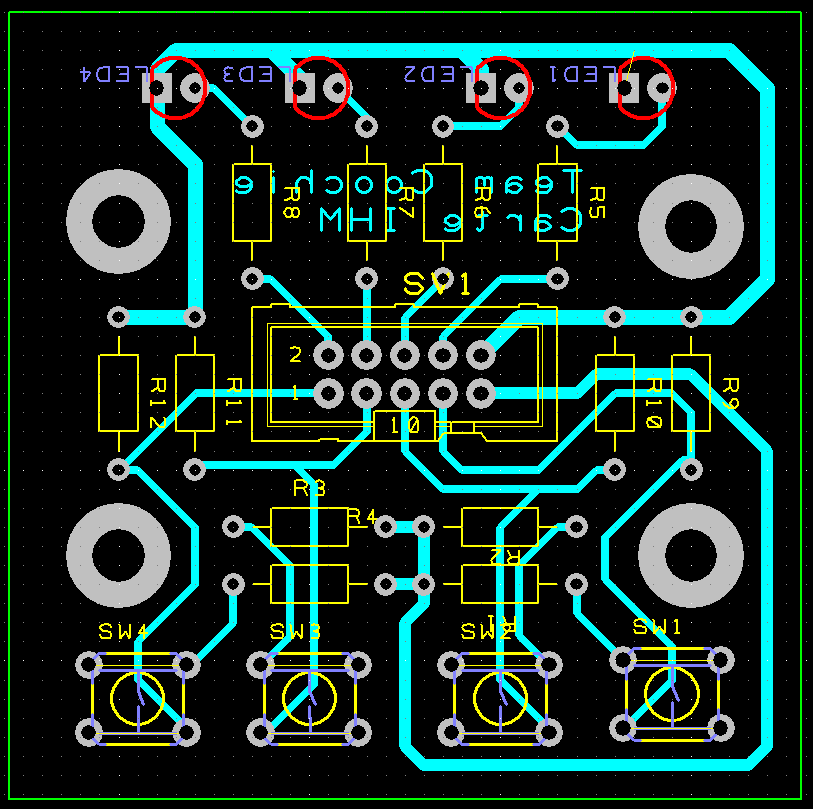
\includegraphics[width=.5\linewidth]{Images/carteIHM_pcb.png}
            \caption{Carte IHM - PCB}
        \label{fig:ihmpcb}
        \end{minipage}
    \end{figure}

\footer{\hfill\insertframenumber/\inserttotalframenumber}
\end{frame}

\subsection{Carte Capteurs}
\begin{frame}
    \frametitle{Carte Capteurs - \textcolor{green}{Terminée}}
    La carte capteurs est équipée de quatre capteurs TCRT5000 et va permettre au robot de s'orienter dans l'espace et de s'adapter aux contraintes imposées (ligne blanche, confettis, ...).

    \vfill
    \begin{figure}[H]
        \centering
        \begin{minipage}{.5\textwidth}
            \centering
            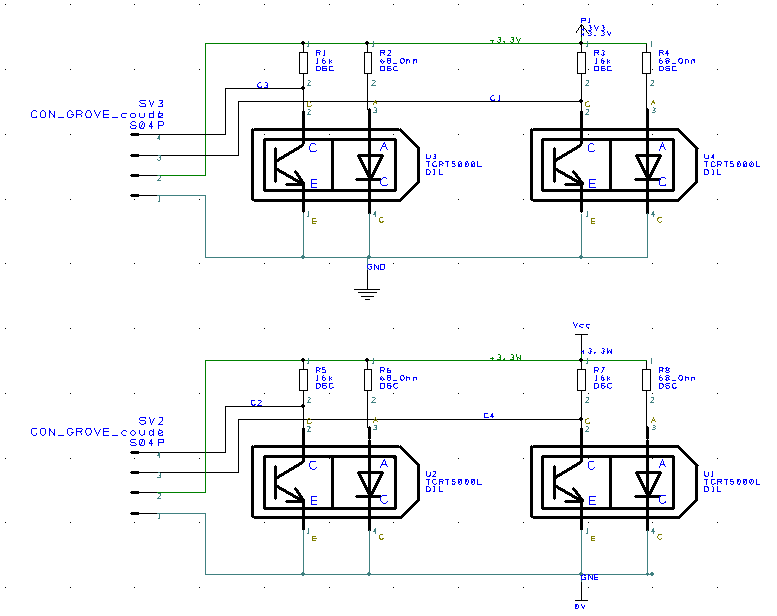
\includegraphics[width=.6\linewidth]{Images/carteCapteurs_sch.png}
            \caption{Carte Capteurs - Schématic}
            \label{fig:capteursch}
        \end{minipage}%
        \begin{minipage}{.5\textwidth}
            \centering
            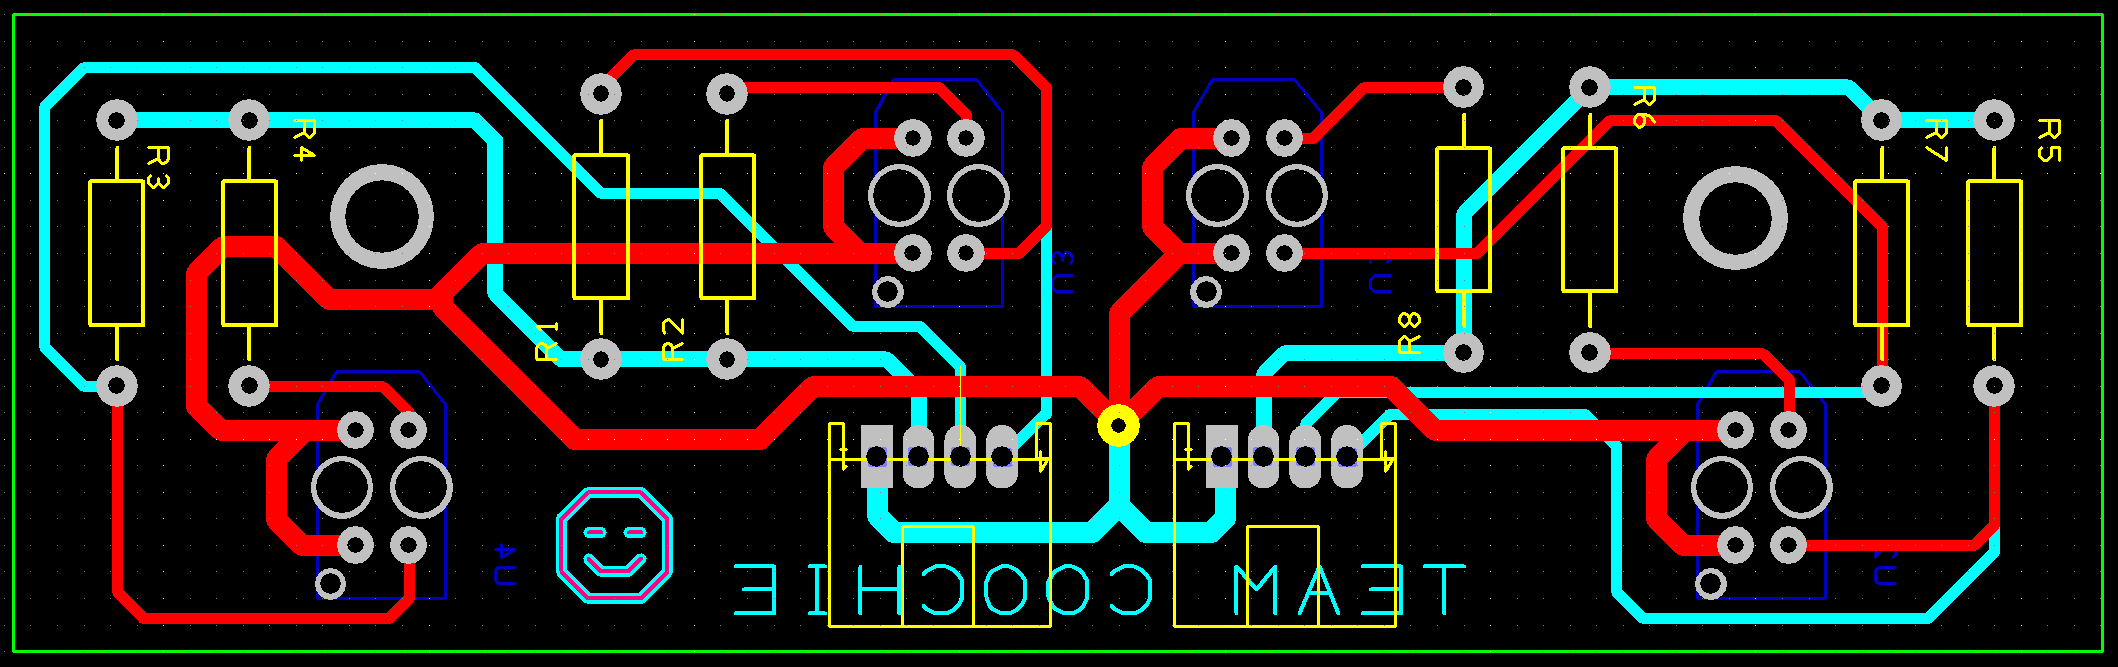
\includegraphics[width=.5\linewidth]{Images/carteCapteurs_pcb.png}
            \caption{Carte Capteurs - PCB}
        \label{fig:capteurpcb}
        \end{minipage}
    \end{figure}

\footer{\hfill\insertframenumber/\inserttotalframenumber}
\end{frame}

\subsection{Carte Hacheur}
\begin{frame}
    \frametitle{Carte Hacheur - \textcolor{red}{En cours}}
    La carte hacheur a pour objectif de contrôler l'activité des moteurs et donc les déplacement du robot. Elle intègre le double pont en H \emph{L298} qui traite les signaux du microcontrôleur pour fournir une tension variable aux moteurs.
    \begin{figure}[H]
        \centering
        \begin{minipage}{.5\textwidth}
            \centering
            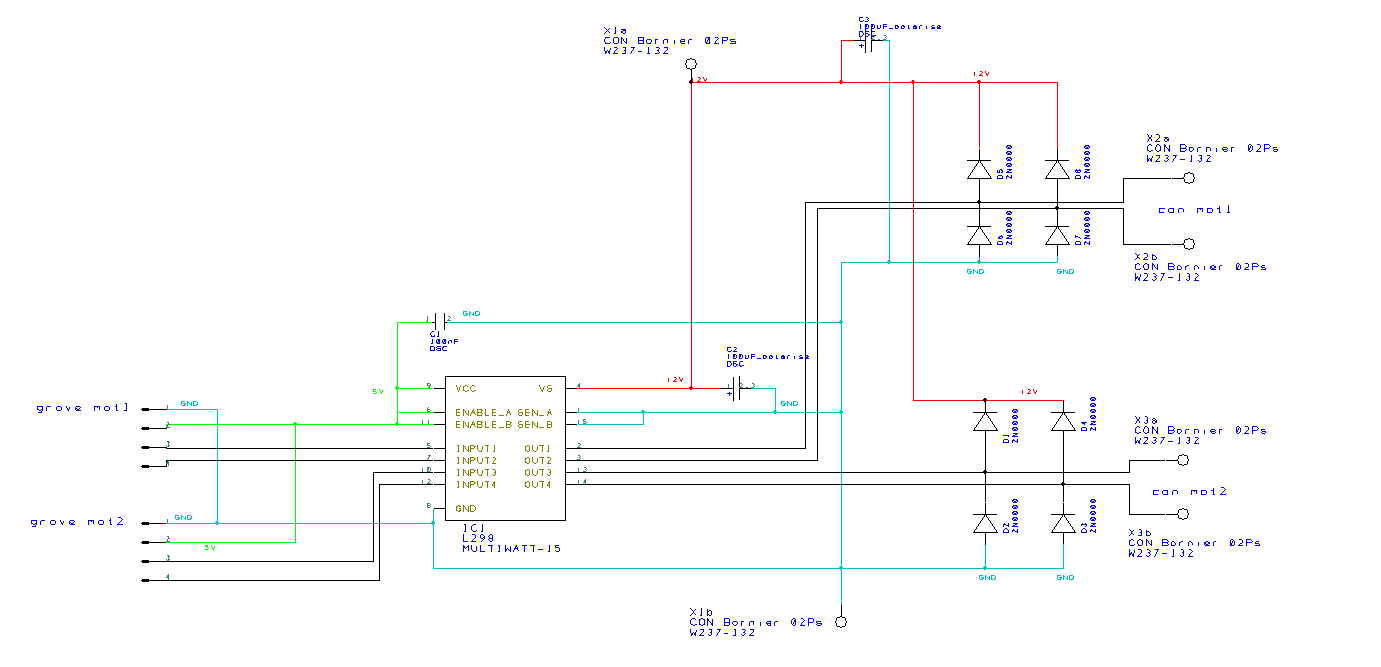
\includegraphics[width=.7\linewidth]{Images/carteHacheur_sch.png}
            \caption{Carte Hacheur - Schématic}
            \label{fig:hacheursch}
        \end{minipage}%
        \begin{minipage}{.5\textwidth}
            \centering
            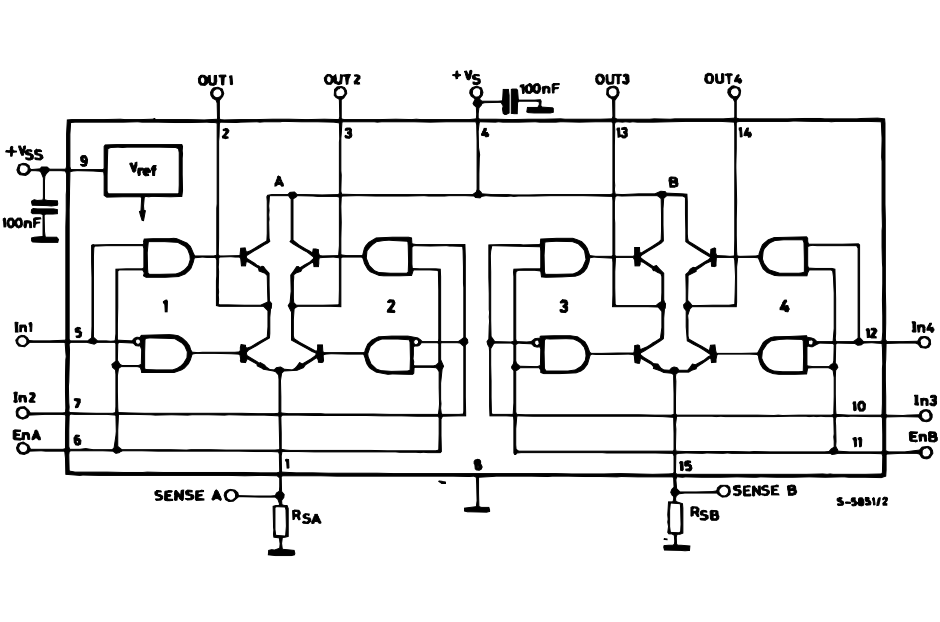
\includegraphics[width=.7\linewidth]{Images/l298.png}
            \caption{Double pont en H \emph{l298}}
            \label{fig:l298}
        \end{minipage}%
    \end{figure}

\footer{\hfill\insertframenumber/\inserttotalframenumber}
\end{frame}

\subsection{Carte Commande}
\begin{frame}
    \frametitle{Carte Commande - Fournie}
    Cette carte, connectée aux pins GPIO du microcontrôleur, rassemble les informations provenant des différents capteurs et distribue les ordres du µC selon le programme sélectionné.

    \vfill
    \begin{figure}[H]
        \centering
        \begin{minipage}{.5\textwidth}
            \centering
            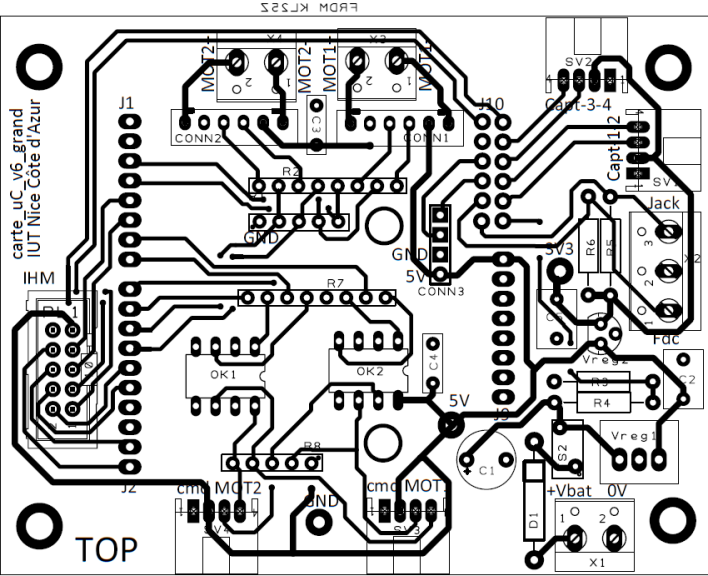
\includegraphics[width=.6\linewidth]{Images/carteCommande_pcb.png}
            \caption{Carte Commande - Schématic}
            \label{fig:commandesch}
        \end{minipage}%
        \begin{minipage}{.5\textwidth}
            \centering
            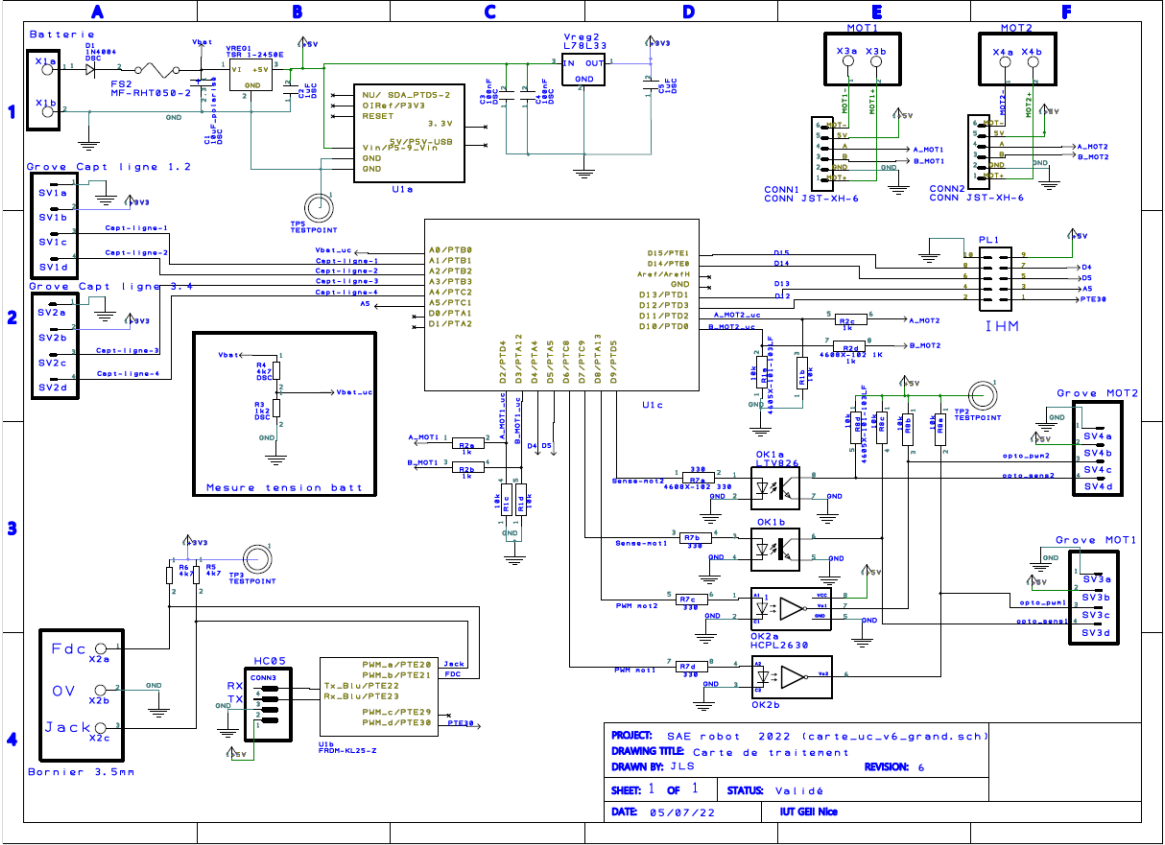
\includegraphics[width=.6\linewidth]{Images/carteCommande_sch.png}
            \caption{Carte Commande - PCB}
        \label{fig:commandepcb}
        \end{minipage}
    \end{figure}

\footer{\hfill\insertframenumber/\inserttotalframenumber}
\end{frame}